% Options for packages loaded elsewhere
\PassOptionsToPackage{unicode}{hyperref}
\PassOptionsToPackage{hyphens}{url}
%
\documentclass[
  11pt,
]{article}
\usepackage{amsmath,amssymb}
\usepackage{iftex}
\ifPDFTeX
  \usepackage[T1]{fontenc}
  \usepackage[utf8]{inputenc}
  \usepackage{textcomp} % provide euro and other symbols
\else % if luatex or xetex
  \usepackage{unicode-math} % this also loads fontspec
  \defaultfontfeatures{Scale=MatchLowercase}
  \defaultfontfeatures[\rmfamily]{Ligatures=TeX,Scale=1}
\fi
\usepackage{lmodern}
\ifPDFTeX\else
  % xetex/luatex font selection
\fi
% Use upquote if available, for straight quotes in verbatim environments
\IfFileExists{upquote.sty}{\usepackage{upquote}}{}
\IfFileExists{microtype.sty}{% use microtype if available
  \usepackage[]{microtype}
  \UseMicrotypeSet[protrusion]{basicmath} % disable protrusion for tt fonts
}{}
\makeatletter
\@ifundefined{KOMAClassName}{% if non-KOMA class
  \IfFileExists{parskip.sty}{%
    \usepackage{parskip}
  }{% else
    \setlength{\parindent}{0pt}
    \setlength{\parskip}{6pt plus 2pt minus 1pt}}
}{% if KOMA class
  \KOMAoptions{parskip=half}}
\makeatother
\usepackage{xcolor}
\usepackage[margin=25mm]{geometry}
\usepackage{graphicx}
\makeatletter
\def\maxwidth{\ifdim\Gin@nat@width>\linewidth\linewidth\else\Gin@nat@width\fi}
\def\maxheight{\ifdim\Gin@nat@height>\textheight\textheight\else\Gin@nat@height\fi}
\makeatother
% Scale images if necessary, so that they will not overflow the page
% margins by default, and it is still possible to overwrite the defaults
% using explicit options in \includegraphics[width, height, ...]{}
\setkeys{Gin}{width=\maxwidth,height=\maxheight,keepaspectratio}
% Set default figure placement to htbp
\makeatletter
\def\fps@figure{htbp}
\makeatother
\setlength{\emergencystretch}{3em} % prevent overfull lines
\providecommand{\tightlist}{%
  \setlength{\itemsep}{0pt}\setlength{\parskip}{0pt}}
\setcounter{secnumdepth}{-\maxdimen} % remove section numbering
\ifLuaTeX
  \usepackage{selnolig}  % disable illegal ligatures
\fi
\usepackage{bookmark}
\IfFileExists{xurl.sty}{\usepackage{xurl}}{} % add URL line breaks if available
\urlstyle{same}
\hypersetup{
  pdftitle={Gravity as the response of recursive field closure},
  pdfauthor={Field Dynamics Research --- research draft},
  hidelinks,
  pdfcreator={LaTeX via pandoc}}

\title{Gravity as the response of recursive field closure}
\usepackage{etoolbox}
\makeatletter
\providecommand{\subtitle}[1]{% add subtitle to \maketitle
  \apptocmd{\@title}{\par {\large #1 \par}}{}{}
}
\makeatother
\subtitle{Proof 26 candidate --- fixed geometry, reversible accounting
and vortex settlement}
\author{Field Dynamics Research --- research draft}
\date{November 2026}

\begin{document}
\maketitle

\section{Abstract}\label{abstract}

We join the geometric convergence of Proofs 23--25 to the earlier
Sierpiński inventory and gravitational-constant calculation. Under
stated closure and address-space premises, a neighboring field must
supply sufficient information for settlement; a 64-address four-child
Triforce ledger admits an exact reversible three-stage Walsh read;
simultaneous order-three label rotation gives 21 independent invariant
contrasts with grades 1, 4, 16; completed blocks cancel their finer
contrasts while retaining inventory. The graded interaction capacity is
273, and a finite-field norm compression of its trace-free subspace
yields the normalized response 17/13. A specified collective
reconstruction observable then equals \((17/13)|t|^{42}\) for common
amplitude gain \(t\). We construct the conditional source and Green
response giving the existing tree-level \(G\) formula if
\(|t|^2=\alpha\) and the microscopic action selects that observable.
Exact fixed-geometry vortex susceptibility demonstrates a candidate
carrier of settlement. The proof establishes the algebraic architecture
and a conditional mechanism, not the physical selection of the source
vertex, gain, or spacetime action. Counterexamples delimit every
inference from counting to dynamics.

\section{1. Premises and inherited
geometry}\label{premises-and-inherited-geometry}

Use
\href{https://github.com/fielddynamics/research/tree/e2b5cd41c63301abad76d9f1881c518dff9cb732/proofs/recursive-triforce-closure}{Proof
23} for the fixed midpoint-lattice, depth-two refinement with 64 paired
face addresses. Use
\href{https://github.com/fielddynamics/research/tree/e2b5cd41c63301abad76d9f1881c518dff9cb732/proofs/flywheel-tetrad-geometry}{Proof
24} for the oriented cycle/row-frame equivalence and actual current
reconstruction, and
\href{https://github.com/fielddynamics/research/tree/e2b5cd41c63301abad76d9f1881c518dff9cb732/proofs/tetrad-flywheel-convergence}{Proof
25} for the common metric and path-independent transport. Their
geometric premises are retained; in particular the regular frame on the
zero-sum space has Gram \(4I-\mathbf1\mathbf1^T\). Chamber coupling is
registered interaction, not a spatial bond between physical TetA and
TetB. The finite address ledger is a fixed mathematical model; the
physical choice of refinement, independent values, and mapping to the
native vortex amplitudes are still hypotheses.

Let \(X=(\mathbb F_2^2)^3\) and \(V=\mathbb R^X\) with counting inner
product. Four labels are identified with \(\mathbb F_4\), choosing zero
as the fixed label of a proper three-cycle. A snapshot \(b\in V\) can
represent occupancy or another registered scalar. Binary occupancy is a
special case. A physical mass is not assumed to equal a number of
occupied addresses. The geometry is held fixed throughout. Define
normalized \(W=H_4^{\otimes3}/8\), where \(H_4(a,b)=(-1)^{a\cdot b}\)
for two-bit labels.

The earlier
\href{https://github.com/fielddynamics/research/blob/e2b5cd41c63301abad76d9f1881c518dff9cb732/research/g_from_topology/g_matrix_synthesis.md}{G
matrix synthesis} already states the target normalization as a ratio of
traces times a determinant. The
\href{https://github.com/fielddynamics/research/blob/e2b5cd41c63301abad76d9f1881c518dff9cb732/research/g_from_topology/read_sweep_synthesis.md}{read-sweep
synthesis} also distributes the exponent as \(7+7+7\). Its total agrees
with \(1+4+16\), but no equality of physical stagewise attenuation
follows: the new decomposition refers to invariant spectral grade
dimensions, and the commuting transforms do not establish clock order.

The physical premises to be tested are: (P1) admissible Field Objects
settle to compatible states, with a sufficient read of neighbors; (P2)
the fixed Triforce register represents the relevant physical
information; (P3) the specified invariant spectral bridge and collective
source are selected by the native action; (P4) a normalized, attractive,
universal scalar long-wave source represents the weak drainless limit.
P1 is sufficient for the abstract necessity theorem; P2--P4 are not
consequences of P1. All exact results below are theorems of the
explicitly defined structures. The word closure does not imply
equilibrium at every instant.

\begin{figure}
\centering
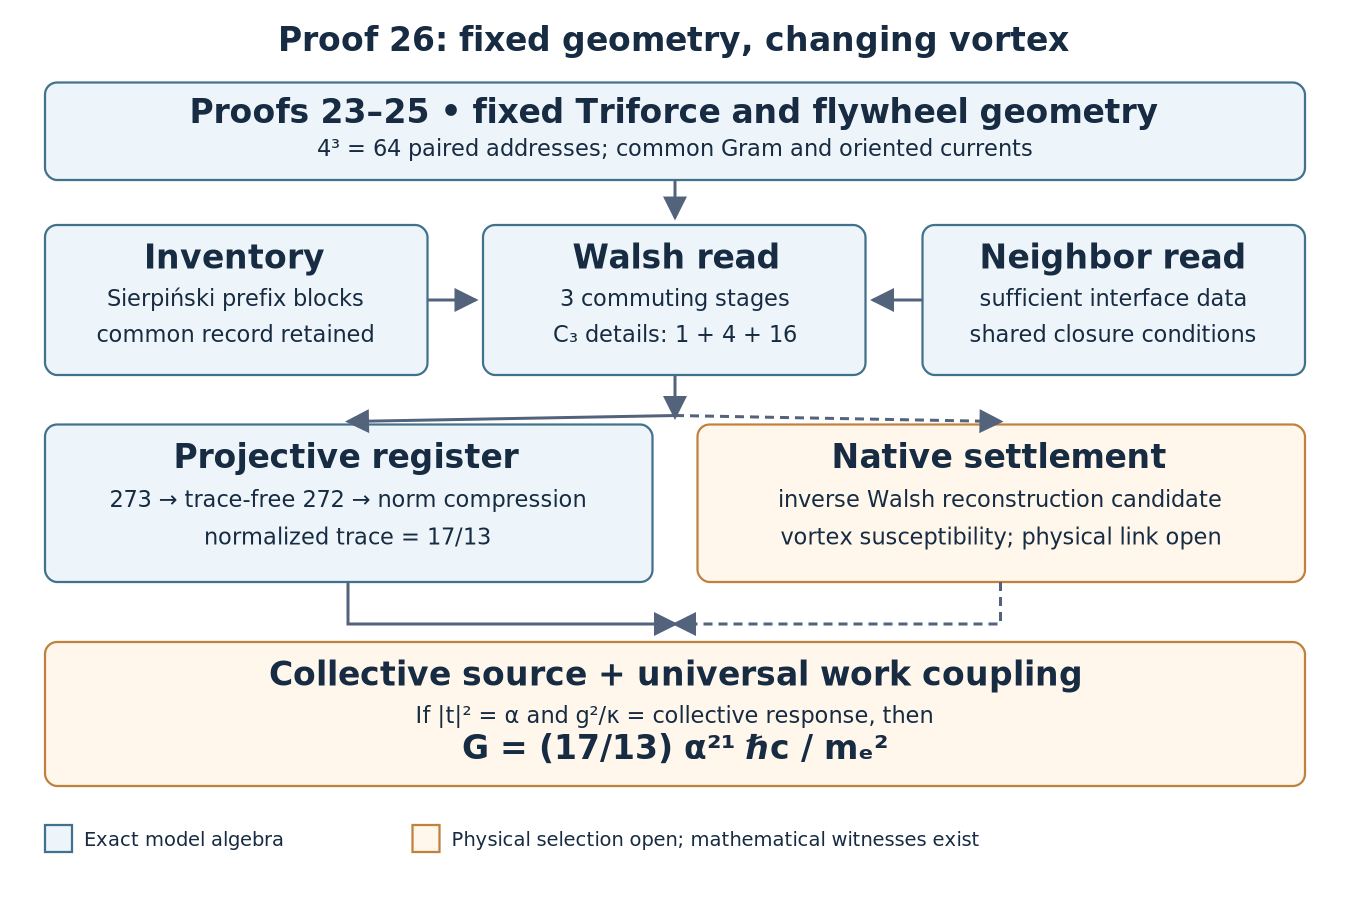
\includegraphics[width=0.92\textwidth,height=\textheight]{figures/proof26_architecture.png}
\caption{Proof architecture: exact algebra and proposed physical
connections.}
\end{figure}

\section{2. Necessity of read and
settlement}\label{necessity-of-read-and-settlement}

\textbf{Theorem 1 (blind closure and sufficient information).} For each
admissible environment \(y\) let \(C_y\) be the feasible closure set of
a Field Object at fixed owned inventory. A blind selection exists
exactly when \(\bigcap_y C_y\ne\varnothing\). If the selected state is
unique, \(S(y)\), a read \(R(y)\) permits exact settlement precisely
when \(R(y)=R(z)\) implies \(S(y)=S(z)\).

\emph{Proof.} A blind selection must be in every feasible set, and a
point of their intersection suffices. In the unique case, a blind
selection exists iff \(S\) is constant. If \(S=F\circ R\), equal reads
have equal outputs. Conversely define \(F\) on \(R(Y)\) by
\(F(R(y))=S(y)\); the implication makes it well defined. For nonunique
feasibility each read fibre must admit a common feasible state. For
differentiable \(S,F,R\), \(DS=DF\,DR\) so \(\ker DR\subseteq\ker DS\)
and \(\operatorname{rank}DR\ge\operatorname{rank}DS\). For linear \(S\)
this bound is attained by coordinates in its image. The rank is a number
of continuous directions, not a count of bits. QED.

\textbf{Theorem 2 (settlement susceptibility).} If \(E(x,y)\) is twice
differentiable, \(E_x(S(y),y)=0\) and \(H_{xx}\) is nonsingular at an
isolated smooth branch, then

\[D_yS=-H_{xx}^{-1}H_{xy},\qquad D_y^2E_* = H_{yy}-H_{yx}H_{xx}^{-1}H_{xy},\]

where \(E_*(y)=E(S(y),y)\). A positive \(H_{xx}\) gives a strict local
minimum; stationarity alone need not.

\emph{Proof.} Differentiate \(E_x=0\) and use the chain rule;
\(D_yE_*=E_y\) since \(E_x=0\). For a quadratic interior energy
\(E=\tfrac12x^TAx+x^TCb+\tfrac12b^TDb-f^Tx\), \(A>0\), the solution is
\(x=A^{-1}(f-Cb)\) and the minimum linear read dimension is exactly
\(\operatorname{rank}C\). The registered energy is
\(\tfrac12 b^T(D-C^TA^{-1}C)b+f^TA^{-1}Cb-\tfrac12 f^TA^{-1}f\). QED.

Thus interaction-sensitive closure requires relevant information, not
necessarily all microscopic records. Mere presence of \(y\) in a formula
does not establish nonblind closure: \((1+y^2)x=0\) has the common
solution \(x=0\). Nor does static dependence imply propagation speed or
a literal algorithm.

\section{3. Fixed address geometry and reversible
read}\label{fixed-address-geometry-and-reversible-read}

\textbf{Theorem 3 (three Walsh sweeps).} The full forward and reverse
Walsh transforms are products of three commuting orthogonal radix-four
stages. Let \(h=H_4/2\). Then

\[W=(h\otimes I_4\otimes I_4)(I_4\otimes h\otimes I_4)(I_4\otimes I_4\otimes h),\quad W^{-1}=W.\]

\emph{Proof.} The two-bit characters satisfy
\(\sum_x(-1)^{(a+b)\cdot x}=4\delta_{ab}\), so \(h^T=h=h^{-1}\). Tensor
multiplication gives the statement. Each full stage has 16 four-point
transforms. The multiresolution tree is a different orthogonal
implementation: deepest sibling reads (16), intermediate common reads
(4), and root read (1), retaining three contrasts at each node. Its 21
readers give 63 contrasts plus one common coefficient. Within each grade
it is related to the Walsh representation by an orthogonal change of
basis, because both give orthonormal bases of the same successive
prefix-detail subspaces. They are not literally the same sequence of
arithmetic operations. QED.

\textbf{Proposition (when the Walsh basis is forced).} A linear operator
commuting with all XOR translations on \(X\) is diagonal in the Walsh
basis. The characters are the simultaneous one-dimensional translation
eigenspaces, hence any commuting map preserves each. Conversely a
diagonal spectral multiplier commutes with every translation. This gives
a mathematical selection criterion, not proof that the physical action
is XOR-translation invariant. Tetrahedral symmetry alone can allow
mixing. No arbitrary physical read is claimed to be Walsh.

\textbf{Theorem 4 (Sierpiński inverse).} Put
\(L=\begin{pmatrix}1&0\\1&1\end{pmatrix}\), \(S=L^{\otimes m}\) in
subset-bit ordering. With \(D_{cc}=(-2)^{|c|}\),

\[H_{2^m}=SDS^T,\qquad H_{2^m}^{-1}=2^{-m}SDS^T.\]

\emph{Proof.} \(S_{ac}=\mathbf1[c\subseteq a]\). Thus
\((SDS^T)_{ab}=\sum_{c\subseteq a\cap b}(-2)^{|c|}=(-1)^{|a\cap b|}\).
Character orthogonality gives the inverse. In particular \(S\) is
unipotent with determinant one, and \(L(z_1)L(z_2)=L(z_1+z_2)\) for the
variable lower shear. Neither one-way sweep nor the unweighted geometry
can supply attenuation. The signed weight and reverse direction are
essential. A conservative paired shear rotation may supply a freely
adjustable gain, but does not select it. QED.

\section{4. Invariant accounting and
registration}\label{invariant-accounting-and-registration}

\textbf{Theorem 5 (projective contrast count).} Let \(g\) multiply every
\(\mathbb F_4\) digit by a primitive element \(\omega\) of order three,
fixing zero. Let \(P_d\) be the orthogonal projection onto functions
depending only on the first \(d\) digits, \(d=0,1,2,3\). The detail
spaces \(V_d=\operatorname{im}(P_d-P_{d-1})\) have dimensions
\(3,12,48\). Their invariant subspaces under \(g\) have dimensions
\(1,4,16\).

\emph{Proof.} Prefix counts give \(\operatorname{rank}P_d=4^d\). There
is one fixed prefix and all other prefixes have orbits of size three.
Invariant dimensions of the prefix spaces are \((4^d+2)/3=1,2,6,22\).
The differences are \(1,4,16\); the commuting projections give an
orthogonal decomposition. In Fourier coordinates the rotation acts
contragrediently (inverse transpose); it preserves the zero digit and
cycles the three others. Its nonzero orbits are the projective points of
\(\mathrm{PG}(2,4)\), after identifying the dual digit action with
scalar multiplication. The 21 orbit sums of characters are independent
and have zero mean. For each orbit, the sum equals
\(4\mathbf1_{\Pi}-1\), where \(\Pi\) is its 16-address common
annihilator; each sum has squared norm 192 and distinct sums are
orthogonal by character orthogonality. QED.

A rotation-invariant scalar observable need not factor through the orbit
average: \(\|(I-Q)b\|^2\) is invariant but is lost under
\(Q=(I+g+g^2)/3\). Thus using only invariant contrasts for physical
settlement requires a sufficiency premise. Also the 21 node readers and
21 invariant contrast directions are not identified individually.

\textbf{Inherited obstruction, checked anew.} P23's physical pointing
sign for \((i,j,k)\) is \((-1)^{[j=i]+[k=i]}\), giving 40 positive and
24 negative leaves. Under the simultaneous three-cycle their invariant
dimensions are 14 and 8. The constant vector has positive/negative
squared weights 40/64 and 24/64. Compressing pointing to the invariant
mean-zero space gives thirteen \(+1\), seven \(-1\), and one \(-1/4\)
eigenvalue (the last follows from the unit vector perpendicular to the
two mean components). This is \textbf{not} the 17-positive/4-negative
abstract depth grading. Moreover simultaneous physical rotation of
ordered cube-corner pairs has four fixed pairs, hence 24 invariants; the
Triforce addresses have only one fixed leaf and 22 invariants. An
equivariant bijection between those representations is impossible. The
present model uses the Triforce addresses, not the physical pair
representation. No physical chamber exchange is inferred from the depth
sign.

\textbf{Theorem 6 (completed-block accounting).} A completed prefix
block \(b_p(w)=\mathbf1[w_{<d}=p]\) has no Walsh coefficient with a
nonzero suffix frequency. If \(b\) is binary with total \(A\), its
unnormalized Walsh coefficients \(c=H_{64}b\) obey

\[c_0=A,\qquad \sum_{a\ne0}c_a^2=64A-A^2.\]

\emph{Proof.} Character sums over each free suffix are zero unless that
frequency is zero. Parseval gives \(\|c\|^2=64\|b\|^2=64A\). Subtract
the constant coefficient. For \(k\) uniform completed cycles plus
residual \(r\), \(H(k\mathbf1+r)=64k e_0+Hr\). A separate pointer
holding completed counts produces the same common record, if the
additive inventory is preserved. QED.

The result holds for any ordering that completes a whole prefix block;
the sequential example is not the earlier global gate-depth ordering at
all occupancies. Nonconstant energy vanishes at empty and full cycles,
hence cannot alone represent accumulated positive mass. The old 0/2/4
landmark score is not the same as a determinant. Nuclear mass number,
signed electrical source, electron configuration and rest energy remain
distinct. Binding energy must be included in the physical mass register.

\section{5. Signed recursive counts and finite-field
compression}\label{signed-recursive-counts-and-finite-field-compression}

\textbf{Theorem 7 (graded count).} On the invariant contrast grades of
sizes \(1,K,K^2\), \(K=4\), define the abstract depth sign
\(D=I_1\oplus(-I_K)\oplus I_{K^2}\). The signed trace and its even
average give \(f(K,s)=1+sK+K^2\), for \(s=+1,0,-1\). The block matrix
algebra
\(\mathcal A=\mathbb R\oplus M_4(\mathbb R)\oplus M_{16}(\mathbb R)\)
has capacity

\[1+K^2+K^4=f(K,1)f(K,-1)=1+K^2 f(K,0).\]

\emph{Proof.} Sum the block dimensions with the stated middle sign;
multiplication cancels the odd powers. Hence 21, 17, 13, 273 and 272
occur in one algebra. A global trace constraint removes one direction,
not one particular cell. The actual lower-triangular Sierpiński blocks
have 91 nonzero entries (1+9+81), not 273, and unit determinant; their
diagonal count is 21. The null-rotation proof's exponential identity
\(\det(\alpha^M)=\alpha^{\operatorname{tr}M}\) for \(\alpha>0\) follows
from \(\det\exp B=\exp\operatorname{tr}B\); it does not identify a
physical source. QED.

\textbf{Theorem 8 (norm-transversal register).} Let \(F=\mathbb F_4\),
\(E=\mathbb F_{64}\), \(L=\mathbb F_{16}\), \(U=\mathbb F_{4096}\). View
\(E\) as a 3-dimensional \(F\)-space and \(U\) as a 3-dimensional
\(L\)-space. Their projective point sets are \(E^*/F^*\) and
\(U^*/L^*\). The norm \(N:U^*\to E^*\) induces a surjection \(\nu\) of
projective point sets with fibres of size 13. The embedded \(E^*/F^*\)
is a norm transversal, and its 13 cosets partition the larger plane into
Baer subplanes.

\emph{Proof.} The subfields intersect in \(F\) (gcd of extension degrees
3 and 2). Norm is \(z^{65}\), restricting to the square on \(E\) and to
the quadratic norm on \(L\). The latter lands in \(F^*\), so the
quotient map is well defined. Squaring is invertible on the order-21
subgroup, proving surjectivity and the transversal property; the order
ratio is 273/21=13. Multiplication by a nonzero element is an invertible
\(L\)-linear map, so every multiplicative coset of the embedded subplane
is a projective image of a Baer subplane. The embedded subplane has the
usual \(F\)-line incidence: an \(L\)-line restricts to at least one
nonzero \(F\)-vector because its one \(L\)-linear constraint yields at
most two \(F\)-linear constraints on three coordinates; if it contains
two independent \(F\)-vectors it contains their \(F\)-line. This
supplies the Baer property. QED.

Choose an \(F\)-basis of \(E\) and \(\theta\in L\setminus F\). Each
projective representative of grade \(d\) has last nonzero coordinate 1
in position \(d\). For same-grade representatives \(u,v\), map
matrix-unit coordinate \((u,v)\) to
\([u+\theta v]\in\mathrm{PG}(2,16)\). Divide by \(1+\theta\) to set the
pivot to 1; every earlier coordinate is uniquely a combination of
\(1/(1+\theta)\) and \(\theta/(1+\theta)\) over \(F\). This proves a
bijection. For \(u=v\) it is \([u]\). The flag and basis are choices;
the map is not an algebra homomorphism or established physical incidence
propagation.

\textbf{Theorem 9 (trace-compressed response).} Let \(M\) be the
21-by-273 norm fibre incidence matrix in the matrix-unit coordinates;
let \(d\) be the vector of the block identity. Then \(MM^T=13I\),
\(Md=\mathbf1\), \(d^Td=21\). Define \(P=I-dd^T/21\), \(R=M/\sqrt{13}\).
The positive compressed operator is

\[B=RPR^T=I-\frac{\mathbf1\mathbf1^T}{273}.\]

\emph{Proof.} The rows of \(M\) have disjoint support of size 13; the
identity is the diagonal transversal. Substitute. Its eigenvalues are 1
(multiplicity 20) and 12/13 (multiplicity 1). Thus
\(\operatorname{rank}P=272\), \(\operatorname{tr}B=272/13\), and

\[\frac{\operatorname{tr}B}{16}=\frac{17}{13}.\]

The determinant of \(B\) is instead 12/13. QED.

The ratio is an exact result of a specified construction, not a proof of
its physical uniqueness. The trace-free restriction, coisometric norm
averaging and normalization by the finest grade are explicit candidate
physical selections. Averaging over all 21 directions instead would
yield \(272/273\). The field norm does not generally preserve incidence.
These qualifications prevent a numerical identity from being mistaken
for dynamics.

\section{6. The proposed gravitational read and its exact conditional
value}\label{the-proposed-gravitational-read-and-its-exact-conditional-value}

Let the spectral bridge act as identity on the constant coefficient and
scalar \(t_j\) on each Walsh grade. In address coordinates

\[J=W^{-1}\Lambda W=\prod_{j=1}^3[I+(t_j-1)(P_j-P_{j-1})].\]

Here the three grades receive their gain once because their projectors
are disjoint. Full contrast determinant has exponents 3,12,48; the
invariant contrast determinant has exponents 1,4,16. Denote the latter
restriction by \(T\). For complex gains use Hermitian adjoints. The
bridge is not idempotent unless each gain is 0 or 1, and is not lossless
unless their magnitudes are one. Distinguish the conservative paired
evolution from its retained output.

\textbf{Theorem 10 (collective response).} Define a formal perturbation
of the complete invariant reconstruction volume,

\[F(\varepsilon)=\det[T^\dagger T(I+\varepsilon B/16)].\]

Then

\[F'(0)=\frac{17}{13}|t_1|^2|t_2|^8|t_3|^{32}.\]

\emph{Proof.} Multiplicativity of determinant and Theorem 9 give
\(F(\varepsilon)=|\det T|^2(1+\varepsilon/16)^{20}(1+12\varepsilon/208)\).
Differentiate at zero. This also holds for singular \(T\) because the
determinant factors even then. In the common-gain case
\(|t_j|^2=\alpha\), the response is \((17/13)\alpha^{21}\). QED.

\textbf{Proposition (testable complete-frame source selection).} Let
\(p_i\) be independent retained intensities in the 21 contrast
directions. If a source observable is a polynomial of degree at most one
in each \(p_i\), is zero whenever any \(p_i=0\), and has value \(c\) at
all \(p_i=1\), it is uniquely \(c\prod_i p_i\). Indeed expansion in
square-free monomials and vanishing on each coordinate hyperplane
removes all monomials missing that coordinate. This is a possible
physical selection criterion for the exponent, not a consequence of
ordinary closure or scalar susceptibility. For instance \(p_1\) is a
legitimate ordinary read, and a shared common gate has joint
transmission \(p\) rather than \(p^{21}\). Even a smooth source with
all-or-nothing zeros can have extra factors unless the multi-affine
condition holds. Atomicity alone is insufficient.

\section{7. Physical carrier: fixed geometry, changing
vortex}\label{physical-carrier-fixed-geometry-changing-vortex}

The atomic inventory work and Paper XIII model TetB packing on the same
four-child structure. Their bound law \(x(1-\mu_b)^2=\mu_b\) and
cumulative sum \(\sum_{i=1}^A\mu_b(i^2)\) vary with occupancy, not the
address geometry. The earlier electric-vortex model proposes outward
response from retained matter; the atomic screening preregistrations
failed their primary criteria, so this is motivation rather than
independent validation. The occupation model's signed source
\(q=n_B-n_A\) is odd and total occupation \(s=n_B+n_A\) even under
exchange. This algebra permits neutral mass response without a signed
electric monopole, but physical charge, mass energy, and the exchange
action require derivation.

Use the native constrained response of the balanced Stage VII branch
(source snapshot and verifier in this package). The fixed metric and
stationary vector are

\[G_m=\begin{pmatrix}3&-1&0\\-1&3&0\\0&0&1\end{pmatrix},\quad x_*=(1/3,1,-4/15)^T,\quad \lambda_*=11/10.\]

The inherited matrices are

\[M_+=\begin{pmatrix}-2&1/2&-2\\-1/2&1&-1\\-5&-1&-89/10\end{pmatrix},\quad M_C=\begin{pmatrix}0&-1/2&0\\-1/2&0&-1\\1&-3&1\end{pmatrix}.\]

Write \(P_*=I-x_*x_*^TG_m/(x_*^TG_mx_*)\), \(b_*=P_*M_Cx_*\),
\(A=-(M_+-\lambda_*I)+(I-P_*)\), \(f=225/1232\). On the
fixed-orientation branch the tangent Hessian is \(-A+h f b_* b_*^TG_m\),
with \(h=F''(\chi_*)\). A candidate neighbor drive adds \(2j u\) to the
Hamiltonian, \(u=\operatorname{Re}(A_{\rm ch}^\dagger C B_{\rm ch})\).
Here chamber amplitudes are denoted with subscripts to avoid confusion
with the tangent stiffness.

\textbf{Theorem 11 (fixed-geometry response in the stated sector).} At a
nonsingular point of the branch, differentiation of stationarity and
normalization gives

\[x'(0)=\frac{A^{-1}b_*}{1-hk},\quad u'(0)=\frac{2k}{1-hk},\quad k=f b_*^TG_mA^{-1}b_*=\frac{42815}{290521}.\]

\emph{Proof.} The tangent equation is \((-A+hf b_*b_*^TG_m)x'+b_*=0\);
apply the rank-one inverse formula. The inherited matrices give
\(A^{-1}b_*=(-430,-296,-2960)^T/11319\) by direct rational substitution.
The normalized overlap derivative is \(2f b_*^TG_m x'\). This proves
nonzero response at unchanged geometry when \(1-hk\ne0\). QED.

The two unperturbed tangent eigenvalues of \(M_+-\lambda_*I\) are
\(-33/5\pm\sqrt{22}\), both negative. A positive rank-one update
preserves negative definiteness exactly for \(h<1/k\) (by conjugating
the positive stiffness with its inverse square root in the metric inner
product). The branch is a local maximum in its specified real tangent
sector below the critical curvature; no minimum-energy gravity sign is
inferred from this branch. In particular the changed central coordinate
is a coherent amplitude, not a proven physical throat radius. The drive
\(j\) is introduced, not derived from the neighbor field. A fixed
Hamiltonian graph need not relax asymptotically; dissipation or energy
transfer and retarded propagation require separate dynamics. The native
model has no independently resolved 64-address amplitudes. No physical
reconstruction operator on its full state has been derived.

\section{8. Hierarchical closure and the conditional G
formula}\label{hierarchical-closure-and-the-conditional-g-formula}

\textbf{Theorem 12 (recursive registration).} In a fixed decomposition
with disjoint owned child interiors and admissible common traces, define
\(\mathcal W_D[f]=\inf_{\Phi|_{\partial D}=f}E_D[\Phi]\). The parent
registered energy is the infimum of the sum of residual and child
registered energies over common interface traces. This follows by
decomposing and gluing admissible fields; when differentiable, variation
of shared traces gives equal and opposite outward work-conjugate flux in
the absence of sheet sources. For a gradient-plus-source action a common
constant boundary shift changes \(\mathcal W_D\) by that constant times
the owned source charge. Internal charges add once, even when physical
influences overlap. No independent attenuation at every hierarchical
level is implied. The scalar boundary functional, not a mass alone, is
generally required to encode tidal response. QED.

\textbf{Theorem 13 (conditional gravitational completion).} Let \(\phi\)
have units of inverse length and \(\rho\) be the mass density, and posit
the local static long-wave action

\[E[\phi]=\hbar c\int\left[\frac{\kappa}{8\pi}|\nabla\phi|^2+g\frac{\rho}{m_e}\phi\right]d^3x,\quad \kappa>0.\]

For decaying boundary data, variation gives
\(\nabla^2\phi=4\pi g\rho/(\kappa m_e)\). The point-source solution
(outside the source) is \(-g m/(\kappa m_e r)\). Eliminating the field
gives the separated pair energy \(-\hbar c g^2 m_1m_2/(\kappa m_e^2r)\);
divergent point self-energies may be removed by using finite disjoint
sources and taking their point limit. The factor of two in the cross
term cancels the one-half in the reduced energy. Thus the force is
attractive and inverse-square with
\(G_{\rm eff}=\hbar c g^2/(\kappa m_e^2)\). QED.

If the native work coupling and stiffness satisfy \(g^2/\kappa=F'(0)\),
and if the common bridge intensity is \(\alpha\), Theorem 10 yields the
existing tree-level formula

\[\boxed{G_{\rm eff}=\frac{17}{13}\alpha^{21}\frac{\hbar c}{m_e^2}.}\]

This is a conditional derivation of the numerical expression from the
geometric response and a continuum source, not an independent
demonstration of the two physical equalities. The candidate mechanism is
that closure adjusts the vortex in the fixed geometry and the
work-conjugate response is gravitational. The scalar \(G\) is the
coupling normalization; local \(\mathbf g=-\nabla\Phi\) is acceleration.
A Lorentz-covariant stress-energy coupling, light propagation,
inertial/gravitational mass equality, drained/drainless rule and
empirical validation are separate requirements. The proposed loop factor
\(1+\alpha/(2\pi)\) is not derived and is not used here.

\section{9. Obstructions and falsifiable next
steps}\label{obstructions-and-falsifiable-next-steps}

\begin{enumerate}
\def\labelenumi{\arabic{enumi}.}
\tightlist
\item
  Scale ambiguity: \(E\mapsto\lambda E\) for positive \(\lambda\)
  preserves stationary states but scales mechanical forces when inertia
  is fixed. Closure does not determine energy units.
\item
  A nonzero mixed Hessian proves local read dependence; it does not
  guarantee distance-dependent reduced energy. For example
  \(E(x,y)=\tfrac12(x-y)^2\) has moving minima and zero reduced energy.
  An ordinary scalar quadratic response through \(T=tI\) is proportional
  to \(|t|^2\), not \(|t|^{42}\). A complete-frame source must be
  derived, not presumed.
\item
  The map \(Q\) can discard relevant anisotropy. A fully filled cycle
  has no detail but retains mass inventory. Derive the physical source
  from the conserved energy, including binding, rather than setting mass
  equal to detail or bare occupancy.
\item
  Translation symmetry is sufficient for Walsh diagonality but is not
  implied by tetrahedral symmetry. Demonstrate a native fine-address
  read or derive it by consistent refinement of the actual Hamiltonian.
  Test whether the physical symmetry selects the intended invariant
  sector; respect P23's representation obstructions.
\item
  Extract the native source vertex by differentiating the action with
  respect to a registered neighbor boundary perturbation. Measure its
  rank, signs, stiffness, cross-mode mixing and response to each blocked
  direction. Check whether every lower-order source term vanishes and
  whether independent gain changes satisfy the complete-frame polynomial
  criterion. Test the 16-normalized trace rather than inserting it.
  Derive \(|t|^2=\alpha\) or independently calibrate it
  electromagnetically, not by fitting measured \(G\).
\item
  Prove physical mass additivity with binding corrections and
  conservation; obtain the static Green limit from a causal microscopic
  action. Use isotopes, neutral systems and different charge states as
  discriminating tests. A static snapshot is not instantaneous
  communication.
\end{enumerate}

\textbf{Conclusion.} The same fixed address structure supports a packing
write, reversible Walsh read, nonlinear settlement and inverse
reconstruction. The geometry, invariant counting, projective
normalization construction, and native example of vortex susceptibility
are algebraically established under explicit premises. The physical
bridge to the existing \(G\) calculation is now a precise, testable
candidate, rather than a claim that counting alone determines gravity.
This is the scope of Proof 26 candidate; no prior proof is amended.

\end{document}
